\chapter{Metáforas para o futuro do Bitcoin}
\label{les:21}

\begin{chapquote}{Lewis Carroll, \textit{Alice no País das Maravilhas}}
\enquote{Sei que alguma coisa interessante sempre acontece\ldots}
\end{chapquote}

Nas últimas decadas, tornou-se evidente que a inovação tecnológica não segue uma tendência linear. Quer você acredite na singularidade tecnológica ou não, é inegável o progresso exponencial em muitas áreas. Não só isso, mas a taxa em que tecnologias estão sendo adotadas está se acelerando, e antes que você perceba o mato no pátio da escola local se foi e seus filhos estão usando o Snapchat ao invés de estar brincando. Curvas exponenciais têm uma tendência de dar um tapa na sua cara antes que você posse vê-las chegar.

O Bitcoin é uma tecnologia exponencial construída em cima de tecnologias exponenciais.
O site \textit{Our World in Data}\footnote{\url{https://ourworldindata.org/}}
mostra lindamente a velocidade crescente de adoção das tecnologias, começando em 1903
com a introdução de linhas de telefone (veja a figura~\ref{fig:tech-adoption}). Telefone fixo, eletricidade, computadores, internet, telefones celular: todos seguem uma tendência exponencial de custo-performance e adoção. O Bitcoin também segue essa tendência~\cite{tech-adoption}.

\begin{figure}
  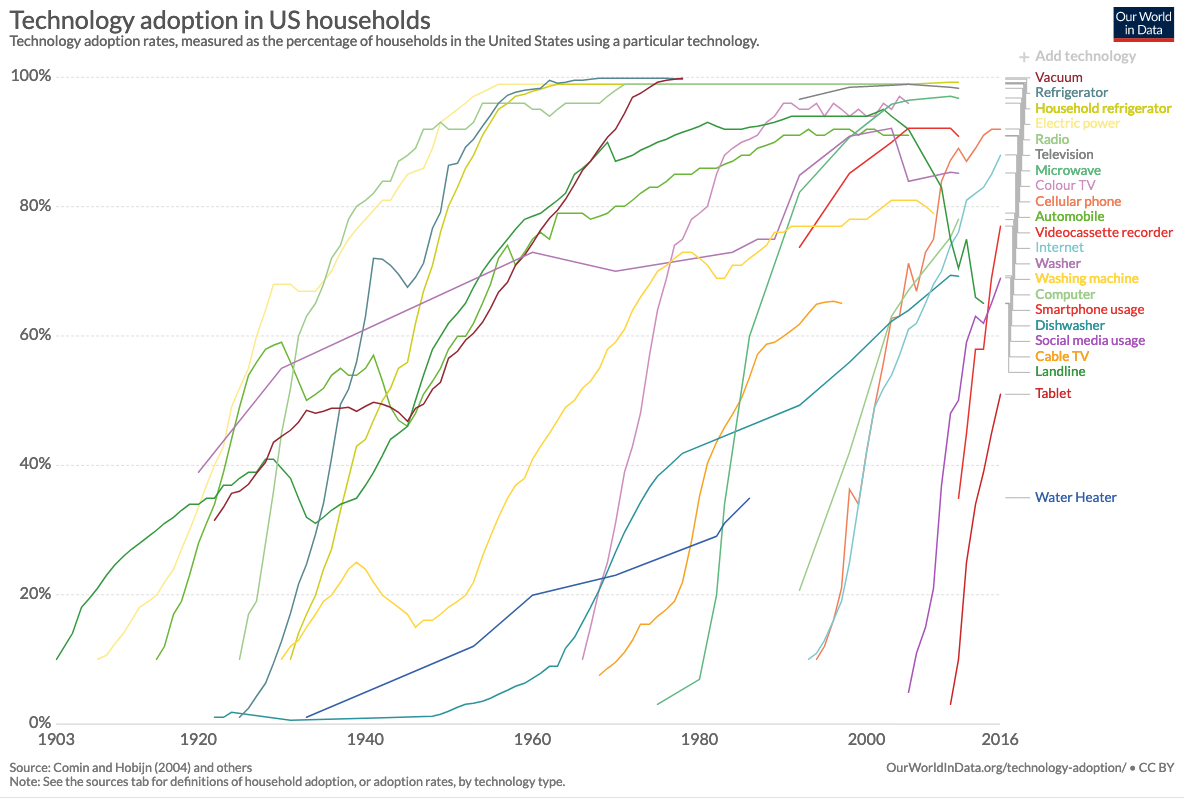
\includegraphics{assets/images/tech-adoption.png}
  \caption{O Bitcoin está literalmente fora dos gráficos.}
  \label{fig:tech-adoption}
\end{figure}

Bitcoin não só tem um, mas múltiplos efeitos de rede\footnote{Trace Mayer,
\textit{The Seven Network Effects of Bitcoin}~\cite{7-network-effects}} todos resultando em crescimento exponencial nas suas respectivas áreas: preço, usuários, segurança, desenvolvedores, fatia de mercado e adoção global como dinheiro.

Tendo sobrevivido a sua infância, o Bitcoin continua crescendo todo dia em vários aspectos.
Claro, a tecnologia ainda não alcançou a maturidade. Talvez esteja na sua adolescência. Mas se a tecnologia é exponencial, o caminho da obscuridade até o uso cotidiano é curto. 

\begin{figure}
  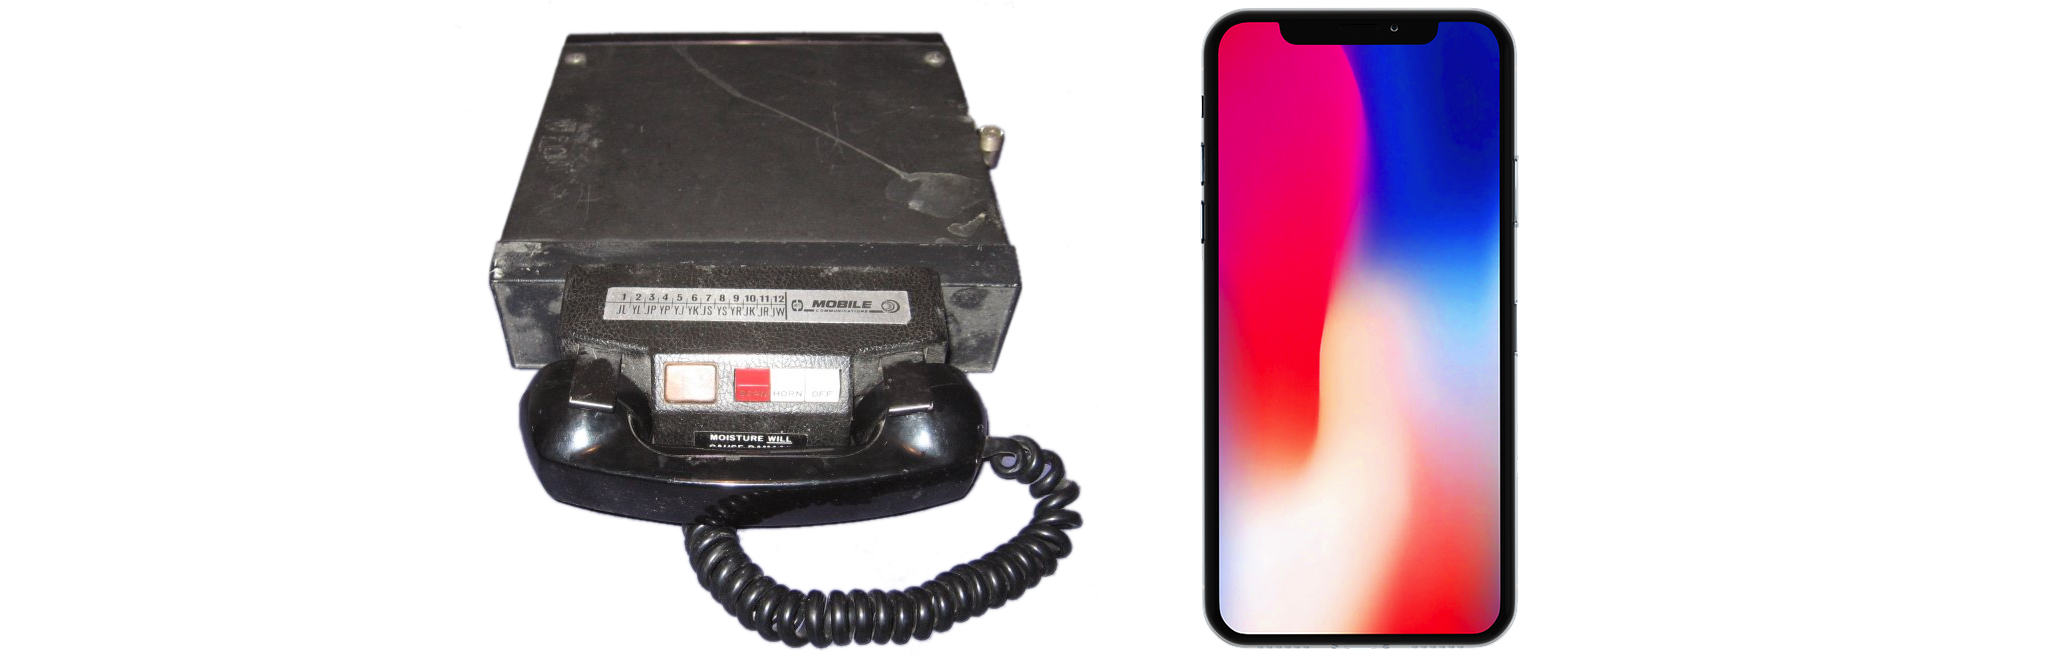
\includegraphics{assets/images/mobile-phone.png}
  \caption{Telefone celular: 1965 vs 2019.}
  \label{fig:mobile-phone}
\end{figure}

Jeff Bezos em sua palestra de 2003 no TED talk, escolheu usar a eletricidade 
como metáfora para o futuro da internet.\footnote{\url{http://bit.ly/bezos-web}} 
Todos os três fenômenos, internet, Bitcoin --- são tecnologias \textit{habilitadoras}, 
redes que habilitam outras coisas. Elas são a infraestrutura pra construir sobre, fundacional por natureza.

A eletricidade já existe há algum tempo. Nós tomamos ela por garantida. A internet é bem mais jovem, mas a maioria das pessoas já a considera por garantida também. O Bitcoin tem apenas dez anos, mas entrou na consciência do público durante a febre do último ciclo. Apenas quem adotou primeiro é quem o toma por garantido. Quanto mais tempo passar, mais pessoas vão reconhecer o Bitcoin como uma coisa que simplesmente é.\footnote{Isso é chamado de  \textit{Efeito Lindy}. O Efeito Lindy é uma teoria onde a expectativa de vida de coisas não-perecíveis, como tecnologia ou uma ideia, é proporcional a sua idade atual, onde cada período de sobrevivência adicional implica em uma expectativa de sobrevida maior.~\cite{wiki:lindy}}

Em 1994, a internet ainda era confusa e não intuitiva. Olhando esse gravação antiga do programa  \textit{Today Show}\footnote{\url{https://youtu.be/UlJku_CSyNg}} nos mostra que o que é natural e intuitivo agora, na verdade, não era no passado. O Bitcoin ainda é confuso e alienígena para muitos, mas assim como a internet agora é uma 'segunda natureza' para os 'nativos digitais', gastar e empilhar sats\footnote{\url{https://twitter.com/hashtag/stackingsats}} vai ser algo cotidiano para os nativos de bitcoin no futuro.

\begin{quotation}\begin{samepage}
\enquote{O Futuro já chegou --- só não está igualmente bem distribuído.}
\begin{flushright} -- William Gibson\footnote{William Gibson, \textit{The Science in Science Fiction} \cite{william-gibson}}
\end{flushright}\end{samepage}\end{quotation}

Em 1995, quase $15\%$ dos adultos americanos usavam a internet. Dados históricos da Pew Research Center~\cite{pew-research} mostram como a internet está emaranhada nas nossas vidas. De acordo com uma pesquisa com consumidores feita pelo Kaspersky Lab~\cite{web:kaspersky}, 13\% dos respondentes usaram Bitcoin e os seus clones para pagar por bens em 2018. Embora pagamentos não sejam o único caso de uso do bitcoin, é uma indicação de onde estamos no tempo da internet: no início para
meados dos anos 90.

Em 1997, Jeff Bezos disse em uma carta para os acionistas~\cite{bezos-letter} que \enquote{este é o dia 1 para a internet}, reconhecendo o poder ainda não explorado do potencial da rede e, por extensão, da sua empresa. Qualquer que seja o dia hoje para o Bitcoin, todo o potencial não explorado é visto por todos, menos aos observadores casuais. 

\begin{figure}
  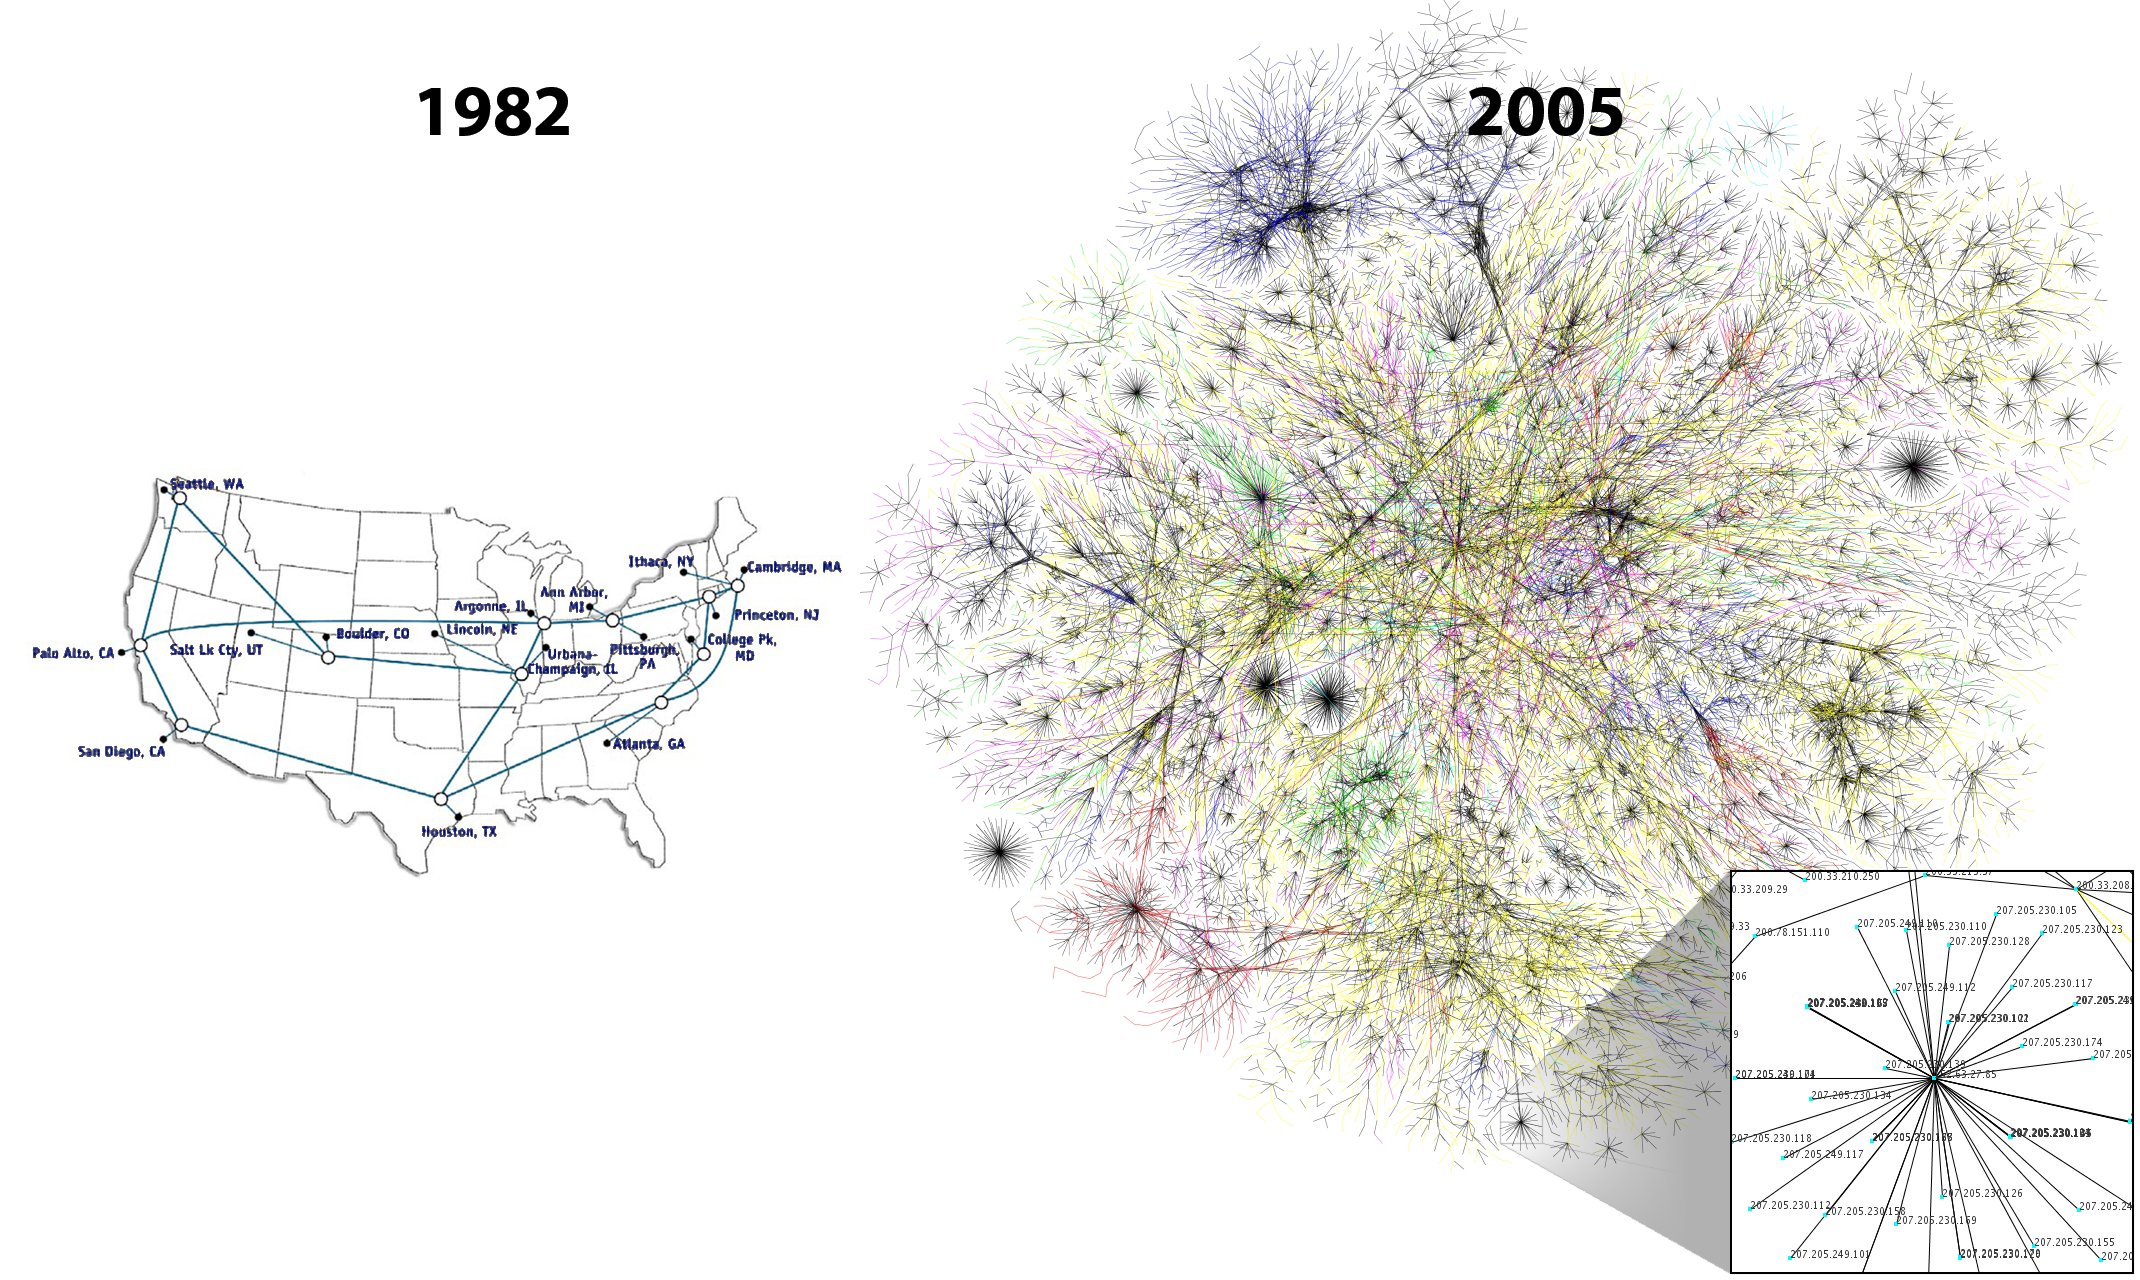
\includegraphics{assets/images/internet-evolution-white-dates.png}
  \caption{A internet, 1982 vs 2005. Imagem sob licença cc-by-sa da Merit Network, Inc. and Barrett Lyon, Opte Project}
  \label{fig:internet-evolution-white-dates}
\end{figure}

O primeiro node de Bitcoin foi ligado em 2009, após Satoshi ter minerado \textit{o bloco gênesis}\footnote{O bloco gênesis é o primeiro bloco da blockchain do Bitcoin. Versões mais modernas do cliente Bitcoin a enumeram como bloco $0$, embora em versões bem iniciais fosse contada como bloco 1. O Bloco gênesis é hardcoded nas aplicações de software que utilizam a blockchain do Bitcoin. É um tipo especial de caso que não faz referência a um bloco anterior e produz um subsídio que não pode ser gasto. O parâmetro \textit{coinbase} contêm, além de dados normais, o seguinte texto: \textit{\enquote{The Times 03/Jan/2009 Chancellor on brink of second bailout for banks}} \cite{btcwiki:genesis-block}} e divulgou o código para o público. O seu node não ficou sozinho por muito tempo. Hal Finney foi uma das primeiras pessoas a entender a ideia e se juntou a rede. Dez anos depois, enquanto eu escrevo, mais de $75.000$\footnote{\url{https://bit.ly/luke-nodecount}} nodes estão rodando o bitcoin.

\begin{figure}
  \centering
  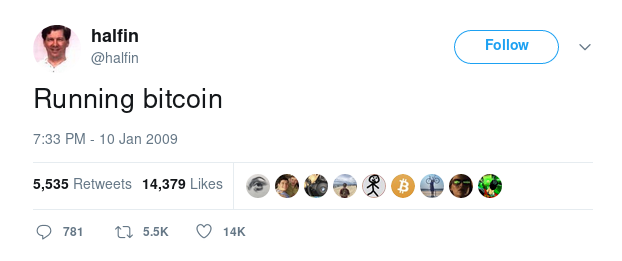
\includegraphics[width=8cm]{assets/images/running-bitcoin.png}
  \caption{Hal Finney escreveu o primeiro tweet mencionando o bitcoin em Janeiro 2009.}
  \label{fig:running-bitcoin}
\end{figure}

A camada base do protocolo não é a única coisa que cresce exponencialmente. A Lightning Network, uma tecnologia de segunda camada, está crescendo a um passo ainda mais rápido.

Em Janeiro de 2018, a lightning network tinha $40$ nodes e $60$ canais~\cite{web:lightning-nodes}.
Em Abril de 2019, a rede cresceu para mais de $4000$ nodes e por volta de $40.000$ canais. Isso tudo ainda sendo uma tecnologia experimental onde perda de fundos podem acontecer. Ainda assim, a tendência é clara: milhões de pessoas são ousadas e estão ávidas para usá-la.

\begin{figure}
  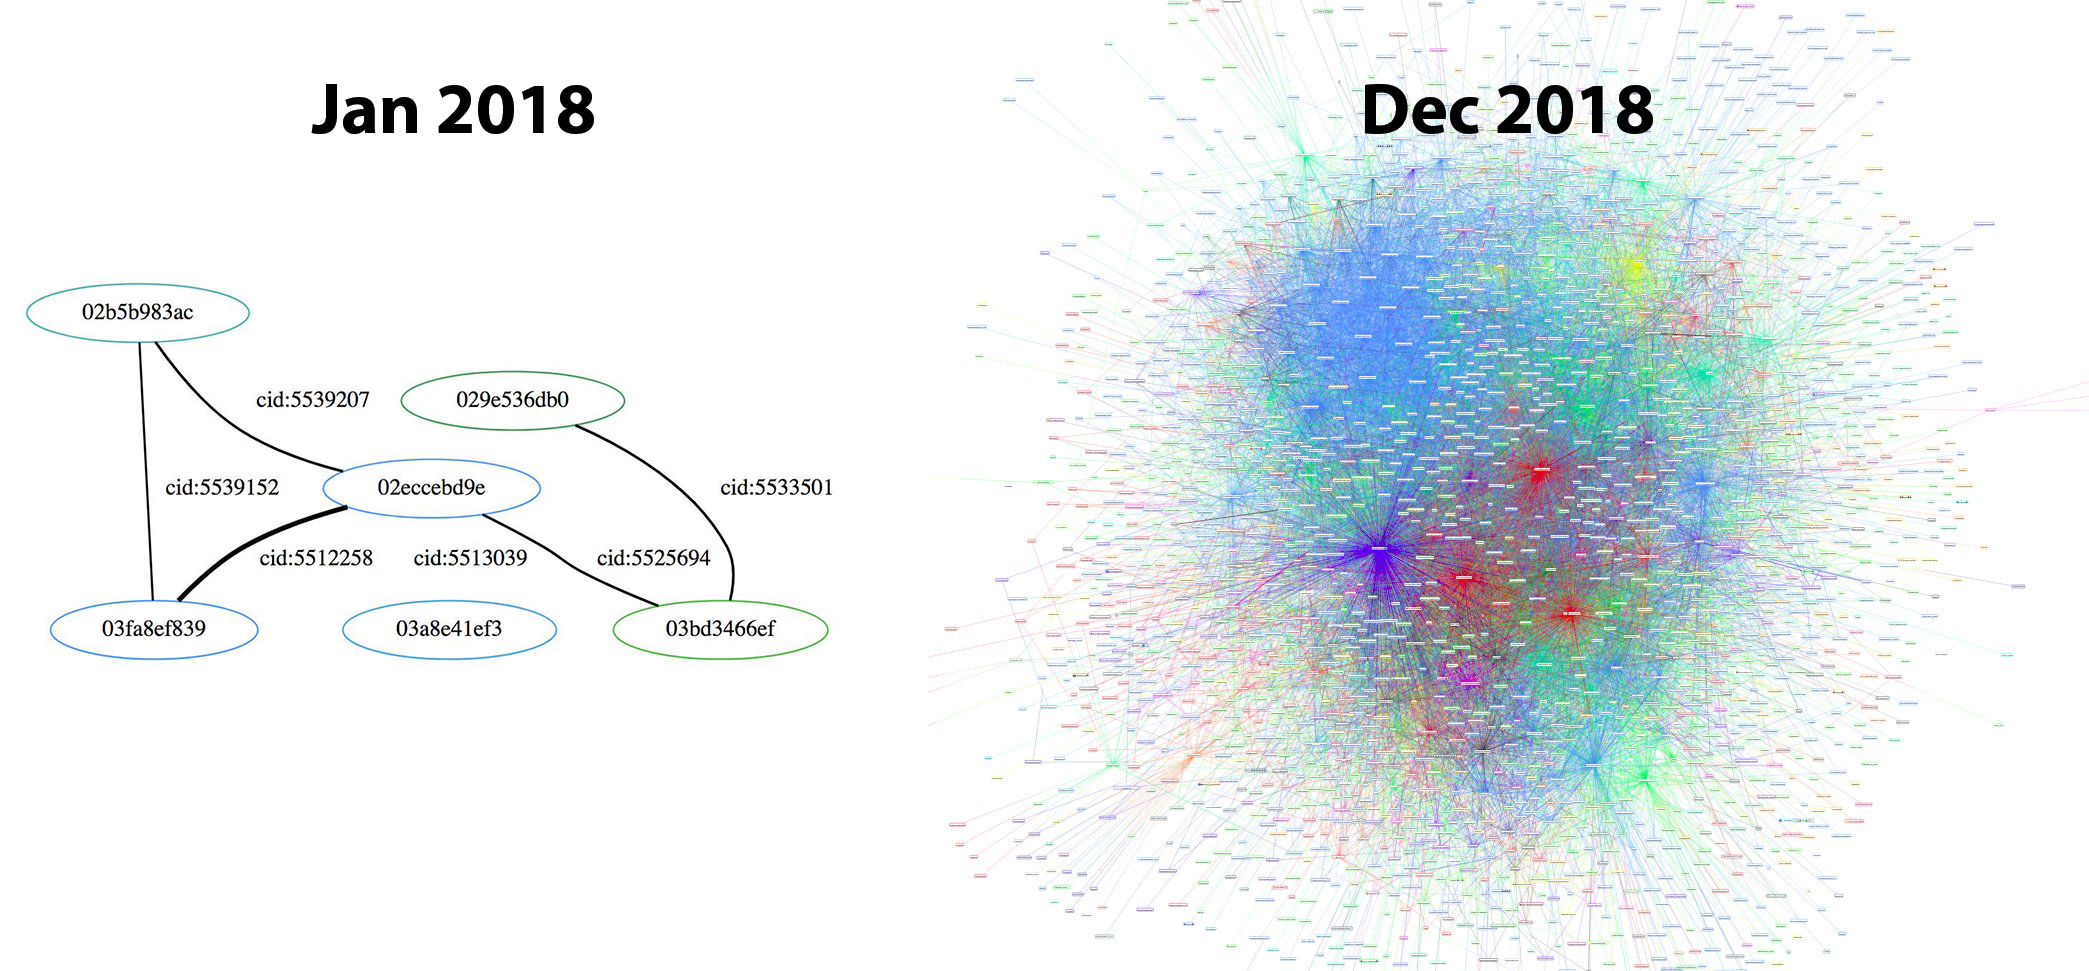
\includegraphics{assets/images/lnd-growth-lopp-white.png}
  \caption{Lightning Network, Janeiro de 2018 vs Dezembro de 2018 Fonte: Jameson Lopp}
  \label{fig:lnd-growth-lopp-white.png}
\end{figure}

Para mim, tendo vivido a subida meteórica da internet, os paralelos entre ela e o Bitcoin são óbvios. Ambos são redes, ambos são tecnologias exponenciais e ambos permitem novas possibilidades, novas indústrias e novos modos de vida. Assim como a eletricidade era a melhor metáfora para entender onde a internet estava indo, a internet pode ser a melhor metáfora para entender para onde o bitcoin vai. Ou, nas palavras de Andreas Antonopoulos, o Bitcoin é \textit{A Internet do Dinheiro}. Essas metáforas ajudam a nos lembrar que a história não se repete, mas muitas vezes rima.

Tecnologias experimentais são difíceis de entender e muitas vezes subestimadas. Mesmo que eu tenha um grande interesse por essas tecnologias, eu sou constantemente surpreendido pela rapidez do progresso e da inovação. Ver o ecossistema do Bitcoin crescer é como ver o crescimento da internet de maneira acelerada. É extremamente estimulante.

Minha busca por tentar entender o Bitcoin me levou para muitos caminhos na história. Entender a estrutura de sociedades antigas, dinheiros do passado e como redes de comunicações se desenvolveram, foi tudo parte da jornada. Do machado para o smartphone, a tecnologia realmente mudou nosso mundo muitas vezes. Tecnologias de redes são especialmente transformadoras: escrita, estradas, eletricidade e internet, todas elas mudaram o mundo. O Bitcoin mudou o meu mundo e vai continuar mudando a mente e os corações de todos os que ousarem usá-lo.

\paragraph{O Bitcoin me ensinou que entender o passado é essencial para conhecer o futuro. Um futuro que apenas começou\ldots}

% ---
%
% #### Down the Rabbit Hole
%
% - [The Rising Speed of Technological Adoption][the rising speed of technological adoption] by Jeff Desjardins
% - [The 7 Network Effects of Bitcoin][multiple network effects] by Trace Mayer
% - [The Electricity Metaphor for the Web's Future][TED talk] by Jeff Bezos
% - [How the internet has woven itself into American life][data from the Pew Research Center] by Susannah Fox and Lee Rainie
% - [Genesis Block][genesis block] on the Bitcoin Wiki
% - [Lindy Effect][more time] on Wikipedia
%
% [Our World in Data]: https://ourworldindata.org/
% [the rising speed of technological adoption]: https://www.visualcapitalist.com/rising-speed-technological-adoption/
% [multiple network effects]: https://www.thrivenotes.com/the-7-network-effects-of-bitcoin/
% [TED talk]: https://www.ted.com/talks/jeff_bezos_on_the_next_web_innovation
% [recording of the Today Show]: https://www.youtube.com/watch?v=UlJku_CSyNg
% [William Gibson]: https://www.npr.org/2018/10/22/1067220/the-science-in-science-fiction
% [data from the Pew Research Center]: https://www.pewinternet.org/2014/02/27/part-1-how-the-internet-has-woven-itself-into-american-life/
% [consumer survey]: https://www.kaspersky.com/blog/money-report-2018/
% [letter to shareholders]: http://media.corporate-ir.net/media_files/irol/97/97664/reports/Shareholderletter97.pdf
% [running bitcoin]: https://twitter.com/halfin/status/1110302988?lang=en
% [40 nodes]: https://bitcoinist.com/bitcoin-lightning-network-mainnet-nodes/
% [reckless]: https://twitter.com/hashtag/reckless
% [Jameson Lopp]: https://twitter.com/lopp/status/1077200836072296449
% [\textit{The Internet of Money}]: https://theinternetofmoney.info/
% [stacking]: https://twitter.com/hashtag/stackingsats
%
% <!-- Bitcoin Wiki -->
% [genesis block]: https://en.bitcoin.it/wiki/Genesis_block
%
% <!-- Wikipedia -->
% [more time]: https://en.wikipedia.org/wiki/Lindy_effect
% [alice]: https://en.wikipedia.org/wiki/Alice%27s_Adventures_in_Wonderland
% [carroll]: https://en.wikipedia.org/wiki/Lewis_Carroll
